\section{Zielsetzung}
\label{sec:Zielsetzung}

Das Ziel dieses Versuches ist es, die Funktionsweise eines Silizium-Halbleiterdetektors und dessen Eigenschaften zu untersuchen. Dazu wird ein Silizium-Streifensensor mit einem Laser und einer $\beta^{-}$-Quelle bestrahlt. Durch die Betrachtung der Ausleseelektronik und die Auswertung der genommenen Daten soll zudem ein Ausblick auf die Funktionsweise und die Arbeit an größeren Teilchendetektoren gegeben werden.

\section{Theorie}
\label{sec:Theorie}
\subsection{Aufbau eines Inneren Detektors am Beispiel des ATLAS Detektors}

Viele der großen teilchenphysikalischen Detektoren, wie z.B. der ATLAS-Detektor am LHC, besitzen einen sogennanten \textit{Tracking Detektor}. Dieser besteht unter anderem aus Silizium-Sensoren, mit denen sich sowohl die Spuren der ionisierenden Teilchen erfassen lassen, als auch die Bestimmung der Impulse dieser ermöglicht wird.\\
Diese Detektorkomponenten werden nahe der Beampipe, in der die Ausgangsteilchen beschleunigt und zur Kollision gebracht werden, angebracht. Die erste Detektorlage bilden dabei die Pixel-Detektoren. Diese besitzen einen sehr ähnlichen Aufbau zu den Streifendetektoren, haben aufgrund ihrer kleineren Größe jedoch eine wesentlich höhere örtliche Auflösung. Durch die hohen Produktionskosten werden um den Pixeldetektor die günstigeren Streifendetektoren in zueinander verdrehten Schichten gelegt, um die Spuren weiter verfolgen zu können. Die letzte Schicht bildet ein Übergangsstrahlungsspurdetektor, dieser ermöglicht die Krümmung der Teilchenspuren bei einem angelegten Magnetfeld zu erfassen und damit die Ladungsbestimmung des Teilchens. Durch das Magnetfeld werden die Teilchenflugbahnen jedoch bereits in den Pixel- und Streifendetektoren gekrümmt wahr genommen. Im weiteren Schritt werden die Krümmungsradien der Teilchenspuren berechnet und daraus die Impulse bestimmt.

\subsection{Halbleiter}
\label{sec:Halbleiter-Theorie}
Halbleiter sind jene Materialien, die weder isolieren noch leiten. Das bedeutet, dass sie eine Bandlücke mit maximal \SI{4}{\electronvolt} bis \SI{5}{\electronvolt} bei Temperaturen $T \neq 0$ besitzen. Die Bandlücke bezeichnet die Energie, die ein Elektron besitzen muss, um von dem Valenz- in das Leitungsband zu wechseln.\\
In diesem Versuch wird der Halbleiter Silizium verwendet. Dieser besitzt vier
Valenzelektronen und eine typische Bandlücke von \SI{1.12}{\electronvolt} \cite{chemie}. Dabei ordnen sich die Siliziumatome in einer Diamantstruktur an, wodurch jedes Atom vier Nachbaratome besitzt, welche alle zur Bindung
beitragen.\\
Beim dem Übergang eines Elektrons in das Leitungsband wird es zu einem freien Elektron und hinterlässt einen positiv geladenen Atomrumpf. Diese positive Restladung wird \textit{Loch} genannt und als Quasiteilchen betrachtet. Trifft nun ein freies Elektron auf ein Loch, so kommt es zu einer Rekombination. Dieser Vorgang wird durch thermische Anregung hervorgerufen, um trotzdem eine geringe Ladungsträgerdichte zu erhalten, wird eine äußere Spannung angelegt. Durch diese lässt sich die Rekombination verhindern und die Elektronen bewegen sich zu der Anode, Löcher hingegen zur Kathode. Dadurch entsteht eine Ladungstrennung und man hat einen Elektronenüberschuss an der Anode und einen Mangel an der Kathode. Durch die Ladungstrennung und das dadurch entstehende elektrische Potential kommt es zur Eigenleitung.
Durch das Hinzufügen von einem geeigneten Fremdatom lässt sich die Leitfähigkeit verbessern. Es wird dabei zwischen p- und n-Typ Halbleitern unterschieden.
Bei p-Typ Halbleitern werden dem Material Akzeptoren hinzugefügt. Dies sind Fremdatome mit einer niedrigeren Anzahl an Valenzelektronen als die des Basisatoms. Dadurch fehlt in der Gitterstruktur zur kovalenten Bindung eine bindende negative Ladung und das Loch bewegt sich wie ein freier positiver Ladungsträger.
Die n-Typ Halbleiter werden hingegen mit Donatoren verunreinigt. Diese zeichnen sich analog zu dem p-Typ dadurch aus, das ein Fremdatom in die Gitterstruktur eingebaut wird. Jedoch besitzt dieses ein Valenzelektron mehr und sorgt daher für eine zusätzliche negative Ladung.\\
Durch Zusammenfügen einer p-dotierten mit einer n-dotierten Schicht innerhalb eines Halbleiters entsteht ein pn-Übergang. Durch die verschieden geladenen Schichten entsteht ein Potentialunterschied mit dem eine sogennante Driftspannung $U_\text{D}$einhergeht, die zu einer Rekombination der Ladungsträger führt. Bei Detektoren wird an die p-Seite ein negatives Potential und an der n-Seite ein positives Potential angelegt. Dies sorgt dafür, dass sich die Ladungsträger zu der Anode/Kathode bewegen und am pn-Übergang eine ladungträgerarme Zone oder Depletionszone ausgebildet wird.
Bei der sogenannten Depletionsspannung $U_\text{Dep}$ ist der Halbleiter zwischen den Kontakten schließlich vollständig depletiert.
Die Depletionsspannung liegt typischerweise wesentlich höher als die
Driftspannung ($U \gg U_\text{D}$), sodass diese vernachlässigt werden kann. Die räumliche Ausbreitung der Depletionszone hängt von der angelegten Vorspannung und der effektiven Dotierungskonzentration
$N_\text{eff}$
\begin{equation}
  N_\text{eff} = \frac{N_\text{D}N_\text{A}}{N_\text{D}+N_\text{A}}
\end{equation}
ab.
Die Parameter $N_\text{D}$ und $N_\text{A}$ bezeichnen die Dotierungskonzentrationen der p- und n-Schichten. Aus den bisherigen Überlegungen folgt die Formel
\begin{equation}
  d(U) = \sqrt{\frac{2\epsilon U}{q N_\text{eff}}},
\end{equation}
mit der Elementarladung $q$ und der Dielektrischen Konstante $\epsilon$ von Silizium. Das Maximum erreicht die Depletionszone bei $U_\text{Dep}$, daher kann auch
\begin{equation}
  d(U) \approx \frac{q}{2\epsilon} N_\text{eff}D^2
\end{equation}
geschrieben werden. Dabei ist $D$ die Sensordicke.\\
Liegt die angelegte Spannung unterhalb $U_\text{Dep}$ gilt für die Dicke der Depletionszone
\begin{align}
  d_\text{c}(U) &= D\sqrt{\frac{U}{U_\text{Dep}}} \hspace{1.7cm}\text{für } U \less U_\text{Dep}.
  \label{eqn:dicke-depletionszone}
\end{align}
Ist die angelegte Spannung allerdings in derselben Größenordnung wie die Depletionsspannung, so folgt für die Dicke der Depletionszone
 \begin{align*}
   d_\text{c}(U) &= D \hspace{3cm}\text{für } U \ge U_\text{Dep}.
 \end{align*}

Um einen Si-Sensor sinnvoll als Detektor einsetzen zu können, sollte er vollständig depletiert sein. Denn durch die entstandende Depletionszone misst die Ausleseelektronik im Idealfall nur dann einen Strom, wenn ein Teilchen durch den Sensor fliegt und durch die deponierte Energie ein Ladungsfluss entsteht.

\subsection{Leckströme}
Der Leckstrom für einen unbestrahlten Sensor wird durch die thermische Anregung von Elektronen aus dem Valenzband in das Leitungsband generiert. Die entstehenden frien Elektronen und Löcher können sich frei bewegen und führen dadurch zu einem Ladungstrom im Sensor, der sich wiederum durch einen kontinuierlichen Lecktrom bemerkbar macht. Für bestrahlte Sensoren setzt sich der Leckstrom aus verschiedenen Komponenten zusammen. Ein Anteil ist der Diffusionsstrom, der durch das Driften von Ladungsträgern im nicht-depletierten Bereich des Sensors erzeugt wird, analog zu den unbestrahlten Snesoren. Der Leckstrom wird durch den \textit{bulk generation}-Strom dominiert, welcher durch Elektronlochpaarproduktion in der Depletionszone erzeugt wird. Diese Elektronenlochpaare werden erzeugt, wenn ein Teilchen durch den Sensor fliegt und dabei Energie deponiert. Der Leckstrom ist linear zum Teilchenfluss $\Phi$, welcher durch den Equivalenzfluss $\Phi_{eq} = \kappa \cdot \Phi$ normiert ist. $\kappa$ ist der individuelle Härtefaktor, der genutzt wird, weil verschiedene Teilchenarten verschiedene Effekte auf die Kristallstruktur des Sensors und damit auch den Leckstrom ausüben.  Der Strom ist zudem linear zu dem Volumen $V_{Dep}$ der Depletionszone und proportional zu einem Faktor $\alpha$, welcher als strombezogene Schadensrate bezeichnet wird.
\begin{equation}
	I = \alpha \cdot \Phi_{eq} \cdot V
\end{equation}

\subsection{Wechselwirkungen ionisierender Strahlung}
In diesem Versuch wird eine ${90}^\text{Sr}$-Quelle verwendet. Diese ist ein reiner $\beta^{-}$-Strahler. Strontium besitzt die Zerfallskette
\begin{equation*}
  {90}^\text{Sr} \stackrel{\beta^{-}}{\longrightarrow} {90}^\text{Y}
  \stackrel{\beta^{-}}{\longrightarrow} {90}^\text{Zr},
\end{equation*}
wobei sowohl Yttrium als auch Strontium nahezu reine $\beta^{-}$-Strahler sind. Deshalb wird ${90}^\text{Sr}$ als Quelle verwendet, da ein relativ reiner Teilchenstrom aus einer Sorte erreicht wird. Strontium besitzt eine Halbwertszeit von $T_{\sfrac{1}{2}} = 28$ Jahren $328$ Tagen und zerfällt danach in Yttrium, welches eine Halbwertszeit von $T_{\sfrac{1}{2}} = 2$ Tagen und $16$ Stunden aufweist \cite{periodensystem}. Dabei zerfallen bei einem $\beta^{-}$-Zerfall Neutronen wie folgt in Protonen:
\begin{equation*}
  \text{n} \rightarrow \text{p} + \text{e}^{-} + \overline{\nu_\text{e}}.
\end{equation*}
Die vorhandene Zerfallsenergie wird auf alle drei Endprodukte verteilt, wobei diese bei \SI{0.546}{\mega\electronvolt} (im Fall \ce{^90Sr}) liegt.

\subsubsection{Wechselwirkung von Elektronen in Materie}
Die Energieverlustcharakteristika von Teilchen legen fest wie sie mit der durchquerten Materie interagieren. Photonen wechselwirken über drei verschiedene Prozesse, die, je nachdem welche Energie das Photon trägt, dominieren. Bei kleineren Energien ist dies der Photoelektrische Effekt, wohingegen zwischen $\SI{30}{\kilo\electronvolt}$ und $\SI{5}{\mega\electronvolt}$ der Compton Effekt überwiegt. Oberhalb dieses Energiebereichs ist die Paarproduktion der dominierende Effekt. Geladene Teilchen haben verschiedene Möglichkeiten um mit Materie zu interagieren. Zum einen ist dies Ionisation, außerdem emittieren leichtere, geladene Teilchen elektromagnetische Bremsstrahlung. Die Hauptwechselwirkungen von schweren Teilchen lassen sich mit Hilfe der Bethe-Bloch-Gleichung beschreiben. Diese fasst unter anderem den Energieverlust durch elastische und inelastische Stöße zusammen, also auch das emittieren von Cherenkovstrahlung.

Bewegt sich ein Elektron in Materie, so führt dieses elastische Stöße mit Kernen und Elektronen durch. Die Energie der durch den $\beta^{-}$-Zerfall induzierten Elektronen ist in diesem Experiment nicht groß genug, um Effekte wie die Bremsstrahlung, die inelastischen Stöße und der Cherenkov-Strahlung auszulösen. Daher werden diese Effekte hier vernachlässigt.

Die Energieabgabe eines Elektrons in einem Halbleiter-Detektor unterscheidet sich somit von schweren geladenen Teilchen. Dabei lässt sich die durchgeschnittliche Energiedisposition durch eine modifizierte Bethe-Bloch-Gleichung beschreiben.
\begin{equation*}
  -\frac{\text{d}E}{\text{d}x} =
  2\pi \text{N}_\text{a} \text{m}_\text{e} \text{c}\rho \frac{\text{Z}}{\text{A}}\frac{1}{\beta^2}
  \left[\text{ln}\left(\frac{\tau^2(\tau + 2)}{2(I\/\text{m}_\text{e}\text{c}^2)^2}\right)
  + \text{F}(\tau) - \delta - 2\frac{\text{c}}{\text{Z}}\right]
	\label{eq:12}
\end{equation*}
In dieser Abwandlung der eigentlichen Bethe-Bloch-Gleichung für Elektronen mit einer Zerfallsenergie von ungefähr \SI{0.5}{\mega\electronvolt} beschreibt $\tau$ die kinetische Energie mit der Einheit $m_\text{e} c^2$. Der Faktor F($\tau$), welcher extra für Elektronen eingefügt wird, ist bestimmt durch:
\begin{equation*}
  \text{F}(\tau) = 1 - \beta^2 + \frac{\tau^2\/8 - (2\text{r}_e + 1) \ln2}{(\tau + 1)^2}
  \hspace{2cm}\text{mit } \tau = \gamma - 1
\end{equation*}
In der Abbildung \ref{fig:tab} ist eine Tabelle der einzelnen Bestandteile der modifizierten Bethe-Bloch-Gleichung dargestellt. Die Elektronen lassen sich jedoch in einem späteren Detektor nicht ausschließlich mit der Energiedeposition in dem inner Tracker identifizieren, dafür werden auch die verschiedenen Kalorimeter gebraucht.

\begin{figure}[htb]
  \centering
  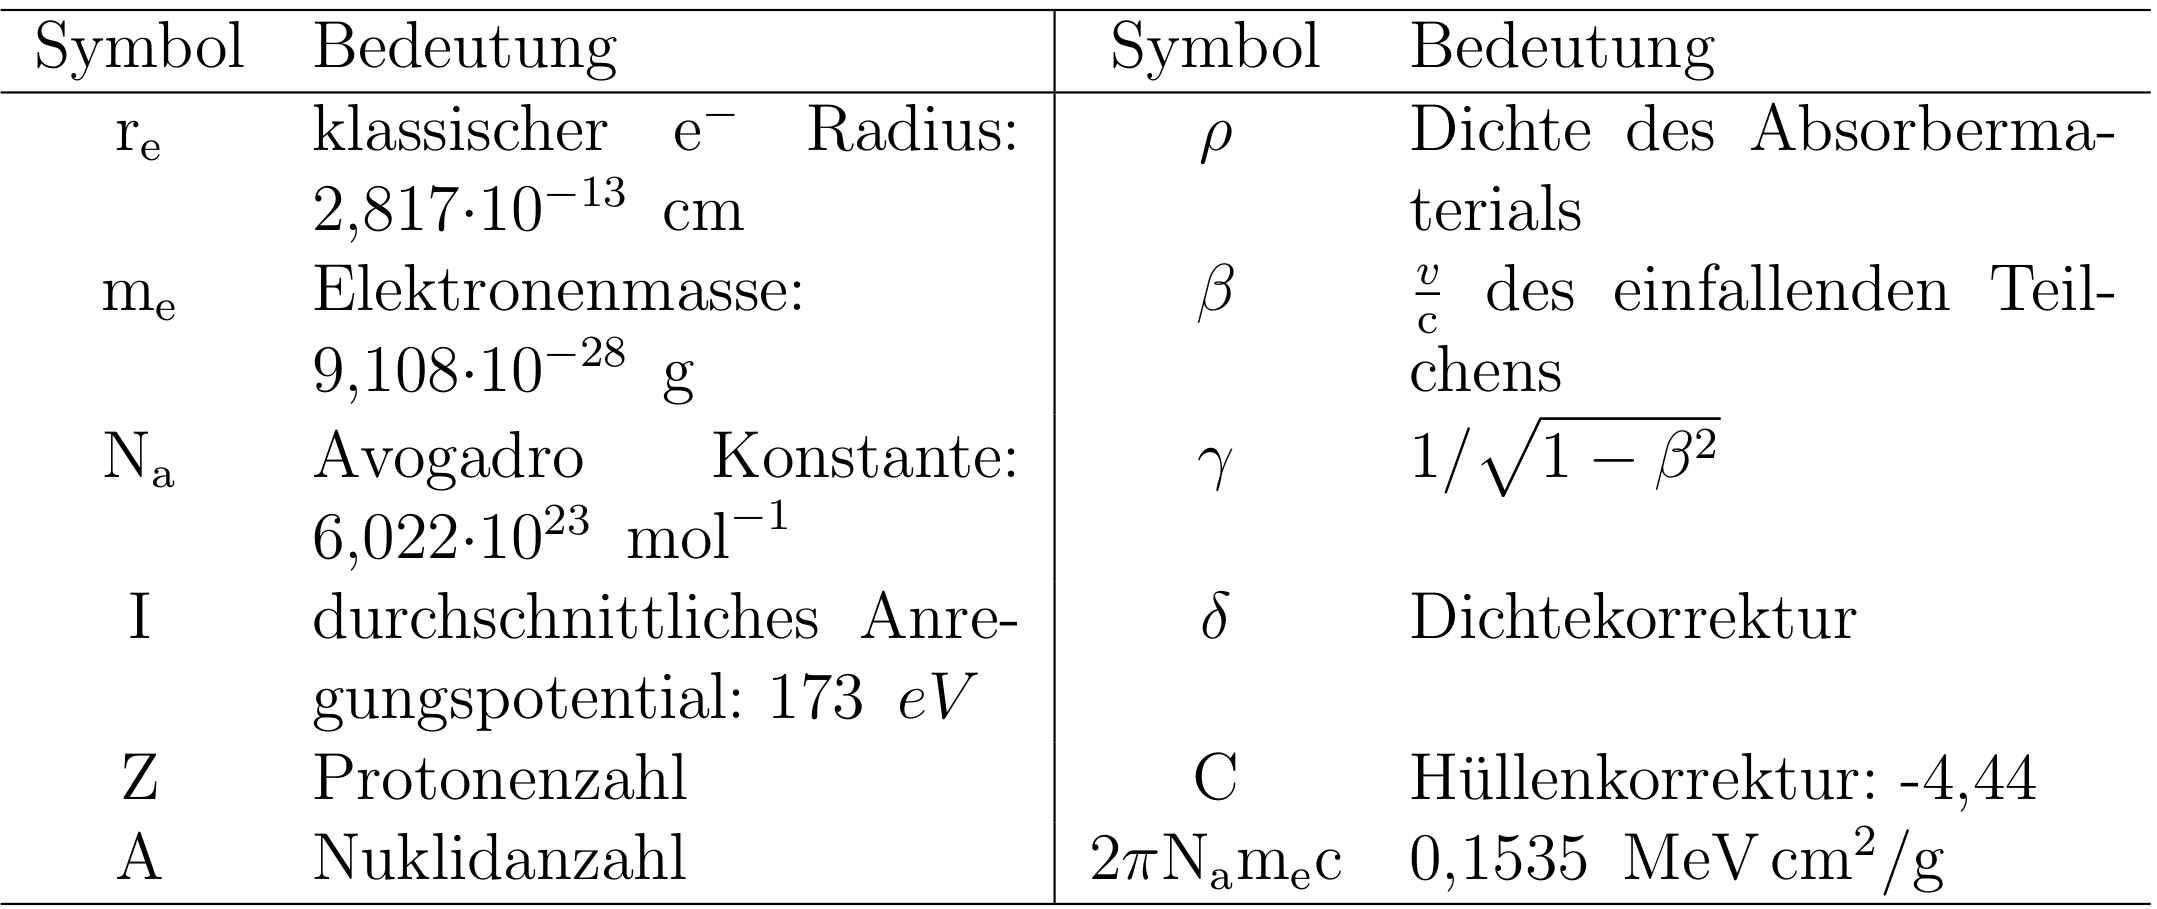
\includegraphics[width=0.8\textwidth]{graphics/Tabelle.png}
  \caption{Bestandteile der modifizierten Bethe-Bloch-Gleichung \cite{anleitung}.}
  \label{fig:tab}
\end{figure}
Typischerweise liegt die Energiedeposition von Elektronen in reinem Silizium bei \SI{3.88}{\mega\electronvolt\per\centi\meter}.

\FloatBarrier
\subsubsection{Energiespektrum im Silizium-Detektor}
Bei hinreichender Dicke des Detektors ist das Spektrum der deponierten Energie eines Elektrons aufgrund des zentralen Grenzwertsatzes durch eine Gaußverteilung gegeben.\\
Der hier verwendete Detektor erfüllt diese Bedingung bei einer Dicke von
\SI{300}{\micro\meter} jedoch nicht. Es gibt nicht genügend Wechselwirkungen
innerhalb des Detektors, um den zentralen Grenzwertsatz anwenden zu können.
Daher entspricht die Verteilung eher einer asymmetrischen Landau-Funktion.
Dies resultiert daraus, dass das eindringende Primärelektron beim Durchqueren des depletierten Sensors entlang seiner Spur Elektron-Loch-Paare produziert. Das neu entstandende Elektron besitzt oft eine höhere Energie und kann mit einem stärker gebundenem Elektron als die Si-Valenzelektronen interagieren. Dieses Elektron wiederum hat oftmals eine höhere kinetische Energie und kann dadurch eine Sekundärionisation hervorrufen. Diese führt zu der asymmetrischen Form des Energiespektrums.\\
Da die Energie der Elektronen des $\beta$-Zerfalls durch eine Verteilung beschrieben werden können, beschreibt das Spektrum der deponierten Energie am besten eine Faltung zwischen einer Gauß- und einer Landau-Funktion. Diese Verteilung ist in Abbildung \ref{fig:faltung} dargestellt.
\begin{figure}[htb]
  \centering
  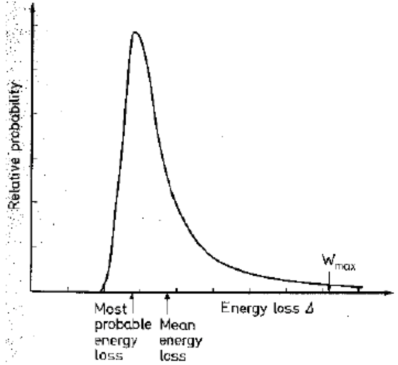
\includegraphics[width=0.5\textwidth]{graphics/Landau.pdf}
  \caption{Spektrum der Energiedisposition eines Elektron in einem dünnen Detektor. \cite{anleitung}}
  \label{fig:faltung}
\end{figure}
Dabei ist zwischen dem mittleren Energieverlust und dem wahrscheinlichsten Energieverlust zu unterscheiden. Dies tritt durch die asymmetrische Landau-Funktion auf.

\FloatBarrier
\subsection{Pedestals und Noise}
\label{sec:Theorie_Noise}
Durch den Detektor und seine Ausleseelektronik enstehen Störsignale bzw. Rauschen, das sogenannte Noise. Um dieses Rauschen zu Minimieren, wird die gemessene Anzahl von Analog-Digital-Converter(ADC)-Counts für ein Signal $k$ und einen Streifen $i$ berechnet durch
\begin{equation*}
  \text{ADC}(i, k) = \text{P}(i) + \text{D}(k) + \text{Signal}(i, k).
\end{equation*}
Dabei beschreibt der Pedestal P($i$) den Mittelwert der ADC-Counts für einen einzelnen Streifen ohne zu erwartendes Signal und der Common Mode Shift D($k$) eine Störung für alle Streifen während eines Events. P($i$) und D($k$) berechnen sich wie folgt:
\begin{align}
  \text{P}(i) &= \frac{1}{N} \sum_{k=1}^N \text{ADC}(i, k)
  \label{eqn:15} \\
  \text{D}(k) &= \frac{1}{128} \sum_{i=1}^{128} \left(\text{ADC}(i, k) - \text{P}(i) \right)
  \label{eqn:18}
\end{align}
Wird nun eine Nullhypothese für das Signal angesetzt (Messung ohne Quelle), so lässt sich durch einen Root Mean Square die Noise der einzelnen Streifen berechnen:
\begin{equation}
  \text{Noise}(i) = \sqrt{ \frac{1}{N-1} \sum_{k=1}^N \left(\text{ADC}(i,k) - \text{P} (i) - \text{D}(k)\right)^2 }
  \label{eqn:16}
\end{equation}
Bei einer Aufnahme von Daten wird ein \textit{Signal-to-Noise-Cut} durchgeführt, um das Rauschen so gut wie möglich herausfiltern zu können. Dies geschieht dadurch, dass ein Verhältnis zwischen den gemessenen Signalen des $\beta$-Strahlers und dem Rauschen der Streifen gebildet wird. Ist dieses Verhältnis größer als 5, so wird ein externer Trigger gesetzt und die Daten werden zur Messung herangezogen. Bleibt das Verhältnis jedoch unter 5, so werden die Daten verworfen.

% \subsection{Clustering}
% \label{sec:Clustering}
% Zuletzt muss noch auf die Bildung von Clustern eingegangen werden. Cluster
% bezeichnen dabei das Messen eines Signals in mehreren Streifen. Grundlegend
% gibt es drei Effekte, die auftreten können.
% \begin{enumerate}
%   \item \textit{Charge Sharing}: Hier trifft ein geladenes Teilchen genau
%   zwischen zwei Streifen auf. Draufhin messen beide Streifen das Signal.
%   \item \textit{Crosstalks}: Durch ein Signal in der Ausleseelektronik wird ein
%   neues Signal an einem benachbarten Streifen gemessen.
%   \item \textit{horizontale Events}: geht ein geladenes Teilchen schräg durch
%   mehrere Streifen hindurch (mit einer Horizontalkomponente $\neq 0$), so gehen
%   jegliche Ortsinformationen verloren. Für diese
%   Ereignisse sind die Streifendetektoren nicht konstuiert worden.
% \end{enumerate}
